%Chapter 4 - MEGA65: A retro revival project
%What is the MEGA6565 project?

\chapter{MEGA65: A retro-computing project}
\label{Chapter4}

This chapter describes and outlines the current state of a retro-computing project, the MEGA65, mentioned in Chapter \ref{Chapter2}. This chapter first provides a description of the MEGA65 project and its intended products. Following the description, a use case study of the MEGA65 is conducted to further describe the MEGA65. The use case study is also employed to elicit the requirements needed to realise the use cases. This detailed information about the MEGA65 project is then used in the next chapter, Chapter \ref{Chapter5}, to evaluate the project against the risk list that was obtained from the case-studies in Chapter \ref{Chapter3}.
%----------------------------------------------------------------------------------------
%----------------------------------------------------------------------------------------
\section{MEGA65 description}
The MEGA65 is a evolution of the Commodore 65, built using FPGA technology at its core, more details are given in section \ref{History of the MEGA65 project}. 

The MEGA65 is planned to have two separate form-factors: a hand-held game console with two cellular modem sockets to allow for telephony, called MEGAphone (figure \ref{MEGAphone concept}) and a desktop form-factor inspired by the look of the Commodore 65, figure \ref{MEGA65 desktop}. 

During development of the MEGA65, the MEGA65 team got into discussions with the Museum of Electronic Games and Art (MEGA) and came to an agreement that MEGA will handle the physical development of the MEGA65 desktop version.

Both form-factors are to have the same FPGA chip and FPGA implementation. This means they are the same computer at the core and can run the same software. Both form-factors are intended to ship with the same software, both custom software made specifically for the MEGA65 and 3rd party software. Both form-factors are collectively referred to as the MEGA65. 

The MEGAphone is to be developed further at Flinders University, with the original MEGA65 team members as well as involving students from the university. The desktop version is to have its physical development handled by MEGA. Physical development refers to the Printed Circuit Board (PCB) (figure \ref{MEGAphone PCB}), the case and the keyboard. 

\begin{figure} \begin{center}
\includegraphics[width=0.5\linewidth]{pics/MEGAphone} 
\end{center} 
\caption{MEGAphone PCB revision 1 populated with most of the components. Top picture is the back of the MEGAphone, bottom is the front. Pictures taken March 2019}
\label{MEGAphone PCB}
\end{figure}

\begin{figure} \begin{center}
\includegraphics[width=0.5\linewidth]{pics/MEGAphone_concept} 
\end{center} 
\caption{MEGAphone design concept. \\
\textit{\small{Picture courtesy of MEGA65.org}}}
\label{MEGAphone concept}
\end{figure}

\begin{figure} \begin{center}
\includegraphics[width=0.5\linewidth]{pics/MEGA65_desktop} 
\end{center} 
\caption{MEGA65 desktop form factor design concept. \\
\textit{\small{Picture courtesy of MEGA65.org}}}
\label{MEGA65 desktop}
\end{figure}


\subsection{MEGA65 team, funding and goals}
As it is relevant to the risk evaluation undertaken in Chapter \ref{Chapter5}, this section will briefly describe the MEGA65 team and funding model. 

The MEGA65 team is centred around Dr. Paul Gardner-Stephen, the inventor and lead contributor to the MEGA65 project. Dr. Paul Gardner-Stephen is a senior lecturer at Flinders University. The MEGA65 project was started as a hobby and the goal of the project is not to generate a profit, as it was in many of the case studies. 

The project is funded, in part, by the university because the project acts as a conduit for student learning. Many of the other project members are volunteers or students.

The MEGA65 project hopes and intends the MEGA65 to be able to function as a secure device and some work has been done to facilitate this.

\subsection{Hardware}
This section briefly describes the hardware, such as the human interface devices of the MEGAphone and desktop form-factor of the MEGA65. 

The desktop form-factor is planned on featuring a built-in 3.5 inch floppy disk drive, like the Commodore 65 prototype. The desktop form factor will also feature a full-size keyboard. It will require a monitor to be connected to view its output. It will also have a SD drive.

It is planned that the MEGAphone will feature its own screen with internal battery and speakers, allowing for mobile usage. The screen will be a touch screen interface with additional controls provided by a d-pad and 4 buttons. The MEGAphone will also feature two sockets for the connection of cellular modems, and the required support to be able to make phone calls and send text messages. It will also have a SD card drive.  

\subsection{Software}
\label{Software}
The MEGA65 has had a range of custom software created for it, this section aims to list and describe that software. This will help further describe the MEGA65 as a product as well as give some explanation of the functions available to these pieces of software which will be helpful to carry out the use case studies.\\

\textbf{Kickstart - the Hypervisor}\\
Kickstart is the name of the hypervisor. It is unusual because it is also like a BIOS and boot-loader in a modern operating system, as well as a hypervisor. It was custom built for the MEGA65 and fits in 16 KB. On start up, the hypervisor loads the BASIC ROM. The BASIC ROM formed the entire operating system on the Commodore 64. Kickstart also handles kernel operations as such it handles all the freeze operations for the Freeze menu. The hypervisor also contains a few utilities housed within FPGA RAM, these can be run from the hypervisor by holding down the two Shift keys on reboot. One of these utilities is a config menu, which allows changing of certain settings. Another is the FDISK utility which can format a SD into the required MEGA65 format, ready for first use.\\

\textbf{The Freeze Menu}\\
The Freeze menu is a program which allows for a variety of useful features. It can be entered into from any program by holding down the Restore key for 1/2 a second, the main menu is shown in figure \ref{freeze menu}. When run, the Freeze Menu stops the current process or freezes it, and saves the state of the computer. This allows programs to be saved and swapped with other programs, then swapped back to, resuming from the original point, this feature is common in modern computers but it wasn't available on the C64. The idea was to get some of the same functionality as a 'freeze cartridge', a popular type of device in the Home Computer era. Some of the features available from the Freeze Menu are:
\begin{enumerate}
\item Restore and return to program which was running when Freeze Menu was run, by pressing F3.
\item Task switching.
\item View, select and load from disk images stored on a SD card.
\item Toggle video mode between NTSC and PAL.
\item Change CPU frequency between pre-set values: 1 MHz (C64 speed), 2 MHz (C128 speed), 3.5 MHz (C65 speed), 40 MHz (MEGA65 speed).
\item Change state of machine such as change register values which store the current amount of lives in a video game. This allows 'freeze cartridge' like 'cheats' to be used.
\item Setting options to set protected ROM and to enable the cartridge port.
\item Allow inspection of memory and allows changes to it. Action replay-like freeze cartridges used features like this to modify games.
\item Audio mixer.
\end{enumerate}


\begin{figure} \begin{center}
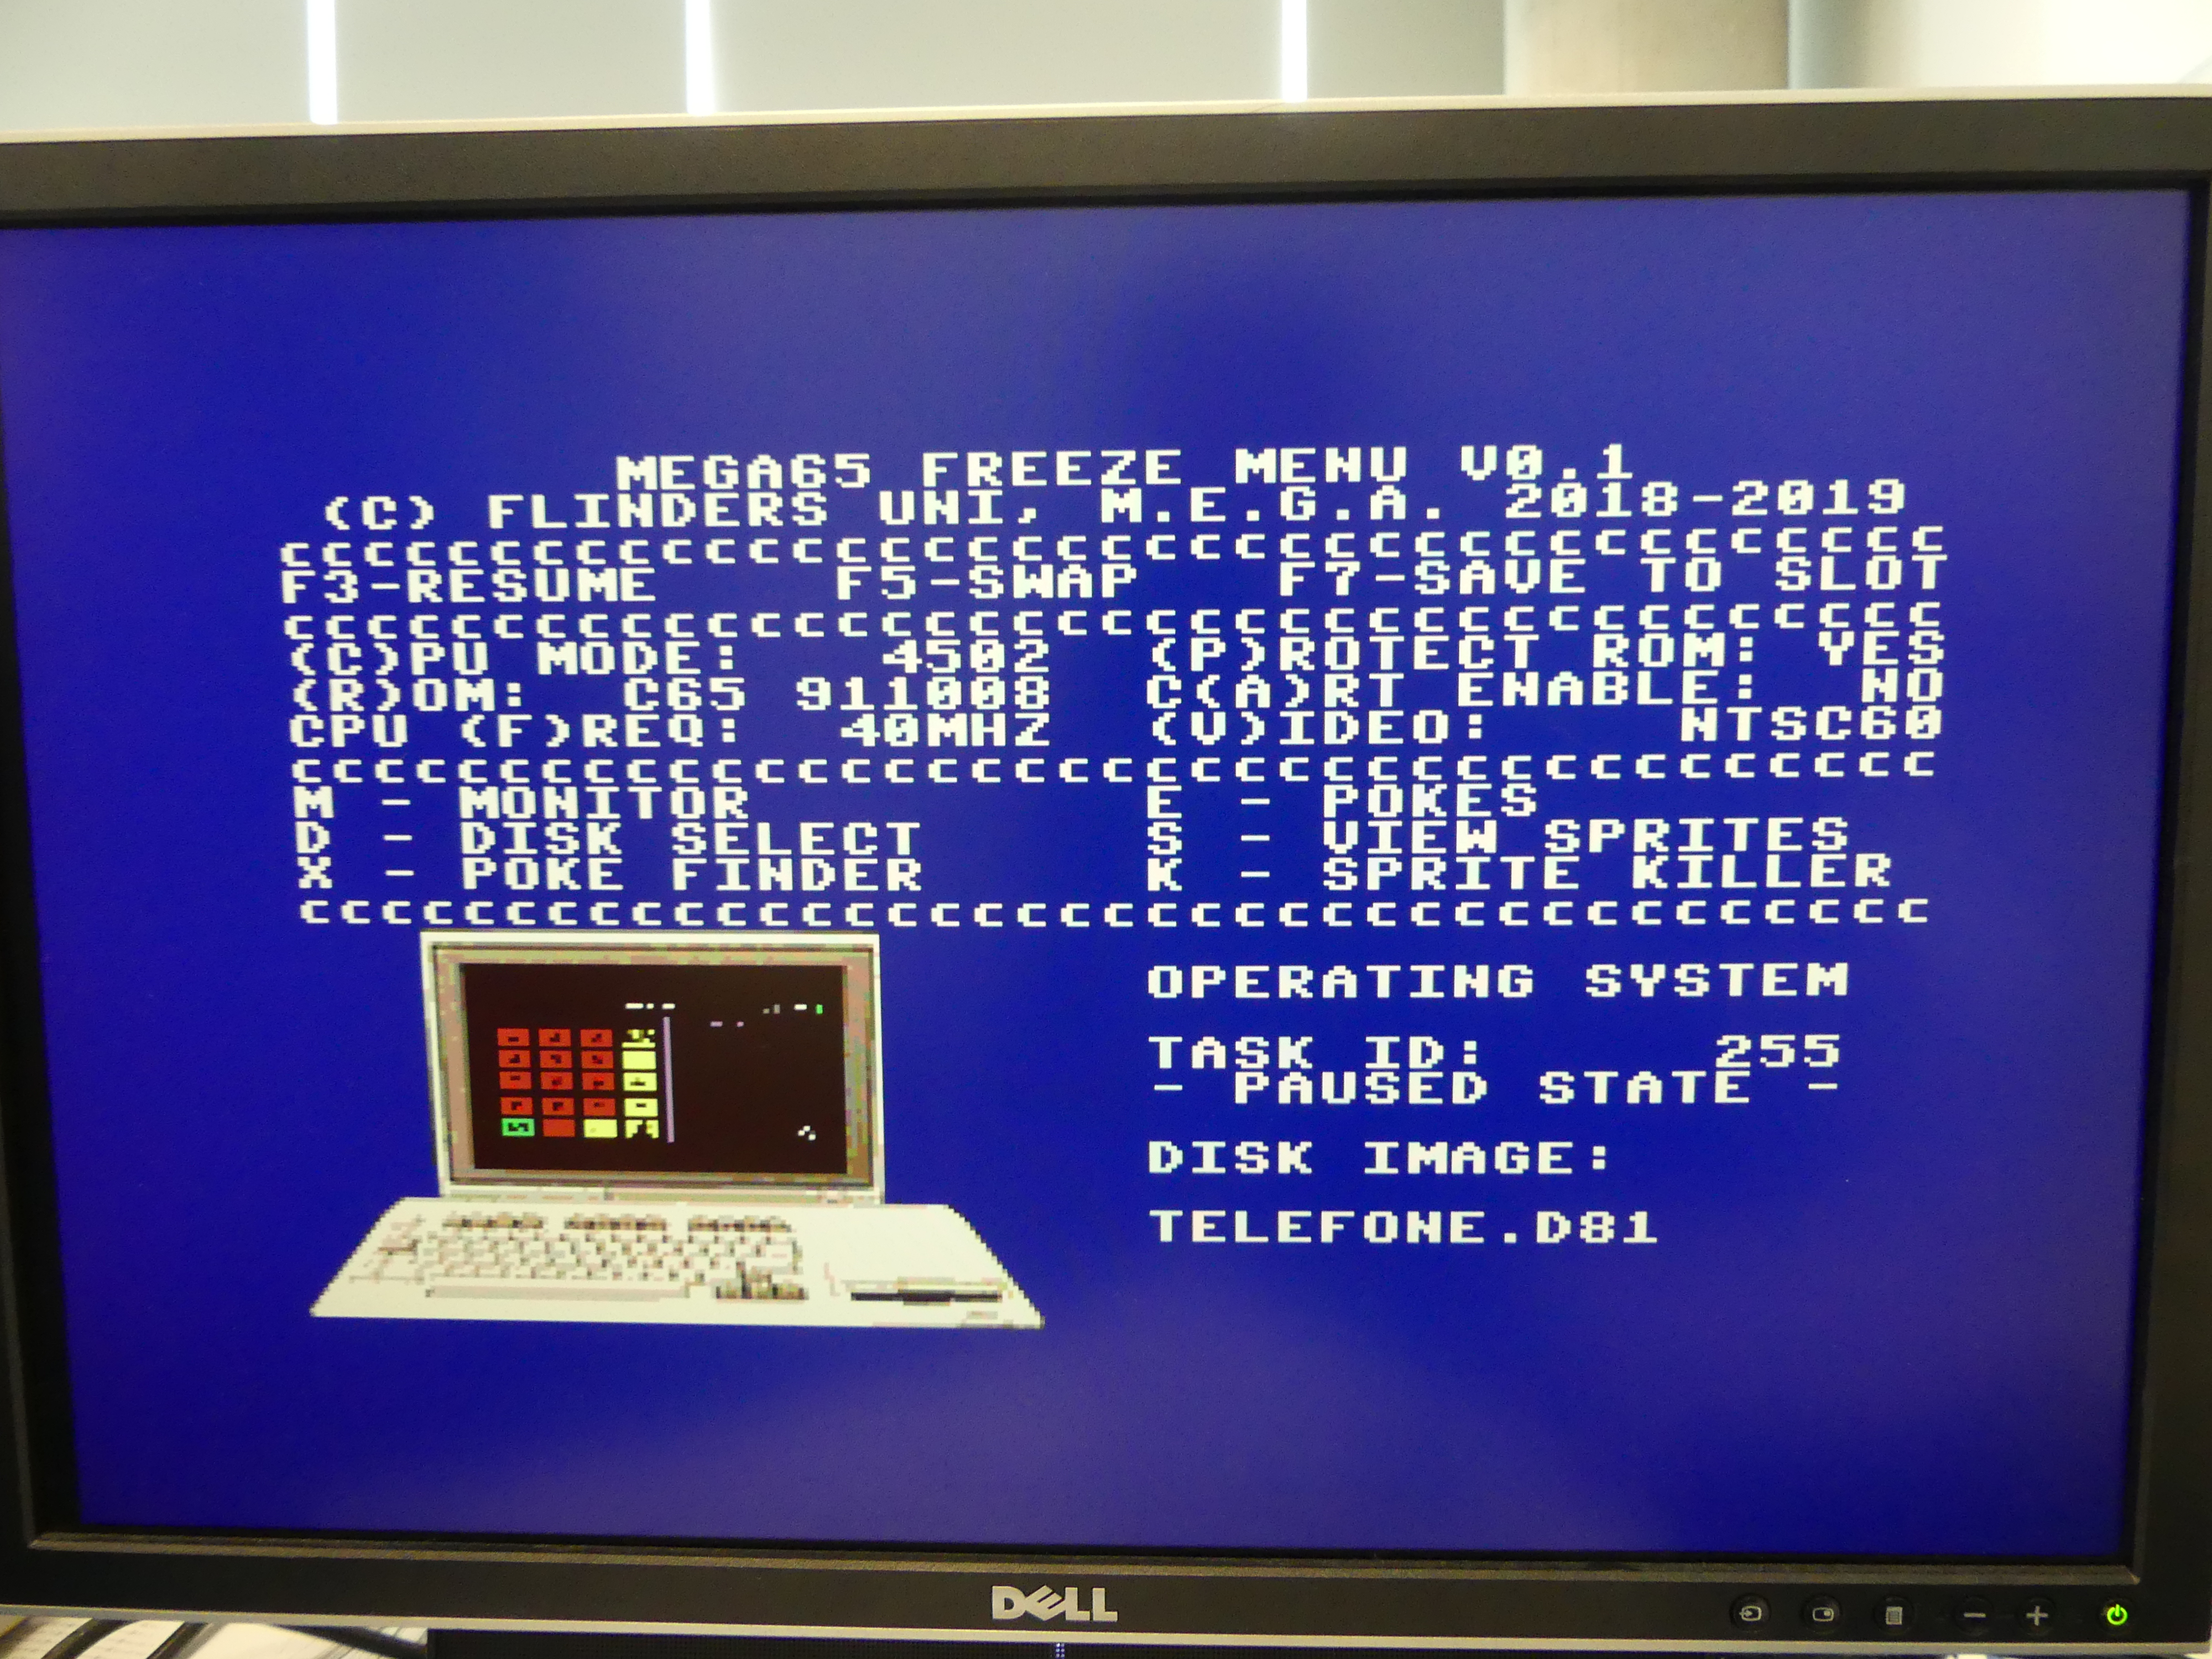
\includegraphics[width=0.5\linewidth]{pics/freeze_menu} 
\end{center} 
\caption{MEGA65 Freeze Menu main screen. \\
\textit{\small{Picture courtesy of MEGA65.org}}}
\label{freeze menu}
\end{figure}

\textbf{Matrix Mode}\\
An out-of-band machine state inspection tool which allows the user to inspect the RAM, ROM, and CPU, I/O registers.\\

\textbf{Secure Mode}\\
Secure mode is a special mode to allow the untrusted components of the MEGA65 to be excluded from the current working environment. This includes the cellular modem and SD card among others. Figure \ref{secure_compartment} shows the secure compartment and the untrustworthy components.\\

\begin{figure} \begin{center}
\includegraphics[width=1.1\linewidth]{pics/secure_compartment} 
\end{center} 
\caption{Secure compartment of the MEGA65. All untrustworthy components are outside of the container.\\
\textit{\small{Picture courtesy of Timothy Kirby}}}
\label{secure_compartment}
\end{figure}

%\textbf{Applications}\\
%This section talks about the application that have been made by MEGA65 project members for the MEGA65. The current plan is for both form factors to be able to run the same software and include the same software on release. There should be no problem with taking the SD card from one machine and running it in the other, as an example.\\

\textbf{MegaWAT} \\
MegaWAT is an open-source slide presentation and editing application \cite{RN163}. It features:
\begin{enumerate}
\item Text editing with colours, attributes and typeface selection
\item Multiple slides
\item Presentation mode
\item Load and save
\item Changeable screen colour
\end{enumerate}

\textbf{MEGA65 IDE}\\
There is also a MEGA65 IDE, which currently only allows viewing of text files. It does currently support viewing of multiple files at once, up to 5 in separate windows, which it can be switched between and the files scrolled through.\\

\textbf{Telephony software}\\
This application allows phone calls to be made over a cellular modem, which the MEGAphone will have sockets to install two of them. \\


\section{Use case study}
This sections lists and discusses several use cases for the MEGA65, in both its form-factors, the desktop computer and the hand-held console. It is hoped that by studying the way the MEGA65 might possibly be used and extracting the features required to fulfil each use case, that a clear description of the MEGA65 can be formed. The requirements can then be used to help capture the current state of the MEGA65 in terms of its development. This list can then help with decision making regarding the minimum viable product for the MEGA65, but that is outside the scope of this thesis. The use cases were first decided upon by determining some roles or actors from the MEGA65's target market, with help from MEGA65 team members. These actors are described below, as well as a brief look at there likely use cases, as seen in Figure \ref{MEGA65_use_cases}.

\subsection{Actors}
\textbf{Gamer}\\
The Gamer's goal is to be able to play retro games. The amount of games available and the ability to add more games to the device are valued by this actor. The ability to use additional HID devices, such as an external joystick is important to this actor.\\

\textbf{8-bit Programmer}\\
The 8-bit Programmer referred to as just Programmer from here on, has a goal of being able to run 8-bit programs in a C64 or C65 environment. They are interested in any feature which will add compatibility between the MEGA65 and C64 or C65 software, such as support for different opcodes or new video modes. \\

\textbf{Technology Enthusiast}\\
The Technology Enthusiast's goal is to try new technology and experience rare or peculiar technological devices, this group also contains 'modders' or 'hackers', people that like to make changes to products they have purchased. They are interested in any of the features but especially in the features that will add something unique or the ability to modify the product easily.\\

\textbf{Privacy Motivated}\\
The Privacy Motivated actor's goals is to be able to securely communicated and carry out a variety of tasks. They are interested in features that will let them thwart any malicious attempts to obtain data. Features that will allow the actor to perform checks on the MEGA65 and thus increase trust of the security of the device, will also be highly valued. \\

\textbf{Educator}\\
The Educator's goal is to teach computer skills and/or topics to others. They are interested in simple computer systems, as this will help highlight the fundamentals of a computer. They are interested in being able to easily write and run code. They are also interested in presenting slides and using 8-bit applications for teaching purposes.\\

\begin{figure} \begin{center}
\includegraphics[width=.6\linewidth]{pics/MEGA65_use_case} 
\end{center} 
\caption{MEGA65 use cases\\}
\label{MEGA65_use_cases}
\end{figure}

\subsection{Use case narratives}
This section describes the use cases in a narrative form. The narrative tries to cover the most likely ways that users will interact with the MEGA65. Where the narrative is for a specific form-factor of the MEGA65 it will be stated, otherwise assume it is for both form-factors. \\


%%%%%%%%%%%%%%%%%%%%%%%%%%%%%%%%%%%%%%%%%%%%%%%%%%%%%%%%%%%%%%%%%%%%%%%%%%%%%%%%%%%%%%%%%%%%%%%%%%%%%%%
\textbf{Play Games}\\
The SD card is physically inserted into the MEGA65 before use, either by the actor or during production. The SD card must contain the games to be played and a version of BASIC which is compatible with the games to be played, e.g. Commodore 64 BASIC is needed to play a Commodore 64 game.

The actors turns on the MEGA65 and then enters the Freeze Menu once the MEGA65 has booted. From the Freeze Menu, the actor navigates to the SD card disk image viewer and loads the image with the desired game on it. While still in the Freeze Menu the actor changes the computer mode to Commodore 64 and then leaves the Freeze Menu. The actor then leaves the Freeze Menu and loads and runs the game from BASIC command prompt. Once the game has loaded, the actor plays the game using the keyboard on the desktop form-factor or the buttons and d-pad (directional pad, 4-way button commonly used on games consoles to control movement) on the MEGAphone form-factor. The actor changes the volume of the game sounds.\\

\textbf{Play Games: Variation}\\
After playing briefly the actor wants to change the CPU mode to the Commodore 64 speed, so the actor enters the Freeze Menu and then changes the CPU mode to the Commodore 64 speed. The actor then leaves the Freeze Menu, resuming the game at the point where the Freeze Menu was entered earlier. 

The actor wishes to control the game using an external joystick. Actor enters Freeze Menu from the game. Actor physically connects joystick via joystick port. Actor resumes game from Freeze Menu and tests joystick, if it works then no more needs to be done, if not, it is most likely that the actor needs to enable the joystick controls from the MEGA65 settings. To do this the actor enters the Freeze Menu and saves the state of the current game being played. Then the actor restarts the MEGA65 and enters the Hypervisor menu and from there the configuration menu and then actor enables the joystick controller option. The actor then leaves the Hypervisor and once the MEGA65 has finished booting, the actor enters the Freeze Menu and loads the saved state of the game they were playing. 

Upon loading the game, the actor notices some strange behaviour in the graphics, they appear to be odd colours and are flashing in a strange way. The actor thinks this is most likely due to the video mode being used is the wrong type for the game. The actor enters the Freeze Menu and changes the display mode from NTSC to PAL and then leaves the Freeze Menu, resuming the game, which now looks as expected.\\

\textbf{Requirements needed to meet narrative}\\
\textbf{Hardware}
\begin{enumerate}
\item SD card slot
\item SD card
\item Power switch
\item Ability to navigate through menus and play games i.e human interface device. For the desktop form-factor this would be a full-sized keyboard. For the MEGAphone form-factor menu interactions, it could be either buttons or a touch screen or both. Playing a game would require the d-pad and at least one button on the MEGAphone.
\item Speaker
\item Volume controllers
\item Joystick port
\end{enumerate}


\textbf{Software}
\begin{enumerate}
\item SD card controller firmware and/or FPGA components to enable reading from SD card
\item Relevant version of BASIC 
\item Game software
\item Freeze Menu - ability to view SD card contents and load images
\item Freeze Menu - ability to enter Freeze Menu from any program
\item Stable MEGA65 FPGA components with ability to boot and run game when supplied with the relevant BASIC ROM
\item Human interface device firmware/drivers created, installed and configured to work with relevant hardware
\item Speaker drivers
\item Volume control drivers 
\item Freeze Menu - ability to change CPU modes to decrease speed to Commodore 64 levels
\item Freeze Menu - ability to "freeze" a program and then reload its state on request
\item Joystick drivers
\item Hypervisor - ability to turn on/off joystick support
\item Freeze Menu - ability to change display mode between NTSC and PAL
\item Video controller capable of doing both NTSC and PAL display modes
\end{enumerate}


%%%%%%%%%%%%%%%%%%%%%%%%%%%%%%%%%%%%%%%%%%%%%%%%%%%%%%%%%%%%%%%%%%%%%%%%%%%%%%%%%%%%%%%%%%%%%%%%%%%%%%%
\textbf{Run 8-bit Application}\\
This use case is practically the same as the Play Games use case except an application is loaded from the SD card not a game. The differences between Play Games use case are: the actor would not want to use a joystick and the application may not need sound. Another difference is the application may be more responsive and faster when the MEGA65 is run at the fastest speed. The MEGAphone would require a keyboard to effectively use most applications.\\

\textbf{Requirements needed to meet narrative}\\
\textbf{Hardware}
\begin{enumerate}
\item SD card slot
\item SD card
\item Power switch
\item Ability to navigate through menus and applications i.e human interface device. For the desktop form factor this would be a full sized keyboard. For the MEGAphone form factor menu interactions, it could be either buttons or a touch screen or both. Controlling an application would require a keyboard.
\item MEGAphone - keyboard port
\end{enumerate}


\textbf{Software}
\begin{enumerate}
\item SD card controller firmware and/or FPGA components to enable reading from SD card
\item Relevant version of BASIC 
\item 8-bit application software
\item Freeze Menu - ability to view SD card contents and load images
\item Freeze Menu - ability to enter Freeze Menu from any program
\item Stable MEGA65 FPGA components with ability to boot and run application when supplied with the relevant BASIC ROM
\item Human interface device firmware/drivers created, installed and configured to work with relevant hardware
\item Freeze Menu - ability to change CPU modes to increase speed
\item Freeze Menu - ability to "freeze" a program and then reload its state on request
\item Keyboard drivers
\end{enumerate}


%%%%%%%%%%%%%%%%%%%%%%%%%%%%%%%%%%%%%%%%%%%%%%%%%%%%%%%%%%%%%%%%%%%%%%%%%%%%%%%%%%%%%%%%%%%%%%%%%%%%%%%
\textbf{Update FPGA bitstream}\\
This use case is unique in that it needs another computer to perform to modifications to the FPGA components. That process will not be covered here as it doesn't relate to the MEGA65 specifically. This use case will start after the FPGA component has been successfully modified.

The actor connects the MEGA65 to the modern computer which houses the updated bitstream via a USB cable. The actor powers the MEGA65 but does not boot it up. The actor then begins the process of copying the new bitstream from the modern computer onto the MEGA65. Once this is complete, the actor disconnects the USB cable then boots up and uses the MEGA65 with the updated bitstream. \\

\textbf{Requirements needed to meet narrative}\\
The requirements relating to the additional computer required to carry out the FPGA modifications are not listed here.\\
\textbf{Hardware}
\begin{enumerate}
\item FPGA USB connection
\item Power switch
\item Ability to navigate through menus and applications i.e human interface device. For the desktop form factor this would be a full sized keyboard. For the MEGAphone form factor menu interactions, it could be either buttons or a touch screen or both.
\end{enumerate}


\textbf{Software}
\begin{enumerate}
\item SD card controller firmware and/or FPGA components to enable reading from SD card
\item Relevant version of BASIC 
\item Freeze Menu - ability to view SD card contents and load images
\item Freeze Menu - ability to enter Freeze Menu from any program
\item Stable MEGA65 FPGA components with ability to boot and run application when supplied with the relevant BASIC ROM
\item Human interface device firmware/drivers created, installed and configured to work with relevant hardware
\end{enumerate}


%%%%%%%%%%%%%%%%%%%%%%%%%%%%%%%%%%%%%%%%%%%%%%%%%%%%%%%%%%%%%%%%%%%%%%%%%%%%%%%%%%%%%%%%%%%%%%%%%%%%%%%
\textbf{Make Phone Call}\\
This use case is only applicable to the MEGAphone form factor, it is assumed there is a 4G cellular modem installed with an active SIM card also installed.

The actor turns on the MEGAphone, after booting the actor enters the Freeze Menu and navigates to the SD card disk image viewer. The actor selects and loads the image with the telephony software on it. The actor then leaves the Freeze Menu and runs the telephony software with a BASIC command. Once the telephony software has loaded, the actor selects a phone number from the saved contacts list. MEGAphone begins a call to the given number, the actor can hear the other person on the call and be heard. The actor adjusts the receiving volume to better hear the other caller.\\

\textbf{Requirements needed to meet narrative}\\
\textbf{Hardware}
\begin{enumerate}
\item SD card slot
\item SD card
\item Power switch
\item Ability to navigate through menus and telephony software i.e human interface device. For the MEGAphone form factor, it could be either buttons or a touch Screen or both. For the desktop form factor a keyboard would be the control method
\item Cellular socket
\item 4G cellular modem
\item Volume controls
\item Speaker
\item Microphone
\end{enumerate}


\textbf{Software}
\begin{enumerate}
\item SD card controller firmware and/or FPGA components to enable reading from SD card
\item Relevant version of BASIC 
\item Telephony software
\item Freeze Menu - ability to view SD card contents and load images
\item Stable MEGA65 FPGA components with ability to boot and run application when supplied with the relevant BASIC ROM
\item Human interface device firmware/drivers created, installed and configured to work with relevant hardware
\item Cellular modem drivers
\item Speaker drivers
\item Microphone drivers
\end{enumerate}


%%%%%%%%%%%%%%%%%%%%%%%%%%%%%%%%%%%%%%%%%%%%%%%%%%%%%%%%%%%%%%%%%%%%%%%%%%%%%%%%%%%%%%%%%%%%%%%%%%%%%%%
\textbf{Securely Communicate}\\
This use case is closely related to the Make Phone Call use case and it is specific to the MEGAphone form-factor.

The actor turns on the MEGAphone and enters the Freeze Menu. From the Freeze Menu the SD image with the telephony software is loaded, then Freeze Menu is left, returning the actor the the BASIC environment. The actor now loads the telephony software from the BASIC environment. The actor has three ways in which they can securely communicate: encrypted phone call, encrypted text message or send an encrypted file via a text message. To achieve any of these the actor uses the telephony software to select the desired communication medium and then selects the option to encrypt the contents. The actor then carries out the phone call or writes and sends the text message. \\

\textbf{Requirements needed to meet narrative}\\
\textbf{Hardware}
\begin{enumerate}
\item SD card slot
\item SD card
\item Power switch
\item Ability to navigate through menus and telephony software i.e human interface device. For the MEGAphone form factor, it could be either buttons or a touch Screen or both. For the desktop form factor a keyboard would be the control method
\item Cellular socket
\item 4G cellular modem
\item Volume controls
\item Speaker
\item Microphone
\end{enumerate}


\textbf{Software}
\begin{enumerate}
\item SD card controller firmware and/or FPGA components to enable reading from SD card
\item Relevant version of BASIC 
\item Telephony software with encryption capabilities
\item Freeze Menu - ability to view SD card contents and load images
\item Stable MEGA65 FPGA components with ability to boot and run application when supplied with the relevant BASIC ROM
\item Human interface device firmware/drivers created, installed and configured to work with relevant hardware
\item Cellular modem drivers
\item Speaker drivers
\item Microphone drivers
\end{enumerate}


%%%%%%%%%%%%%%%%%%%%%%%%%%%%%%%%%%%%%%%%%%%%%%%%%%%%%%%%%%%%%%%%%%%%%%%%%%%%%%%%%%%%%%%%%%%%%%%%%%%%%%%
\textbf{Run Program in Secure Environment}\\
This use case could have many variations but the most important aspects are captured here in a single description, in which the actor wants to type up a new text document then encrypt it, all while being as securer from malicious actors as possible.

The actor turns on the MEGA65, after booting the actor loads their choice of text editing software. The actor then enters "Matrix mode" and requests a secure container to work in, referred to as secure mode in section \ref{Software}. Still within "Matrix mode", the actor inspect the state of the machine for suspicious activity. Leaving "Matrix mode" but still within the secure container, the actor returns to the text editor and types out the document and then encrypts it. The actor leaves secure mode, relinquishing the secure container. \\

\textbf{Requirements needed to meet narrative}\\
\textbf{Hardware}
\begin{enumerate}
\item SD card slot
\item SD card
\item Power switch
\item Ability to navigate through menus and applications i.e human interface device. For the desktop form factor this would be a full sized keyboard. For the MEGAphone form factor menu interactions, it could be either buttons or a touch screen or both. Entering text would require a keyboard.
\item MEGAphone - keyboard port
\end{enumerate}


\textbf{Software}
\begin{enumerate}
\item SD card controller firmware and/or FPGA components to enable reading from SD card
\item Relevant version of BASIC 
\item Text editing software
\item Freeze Menu - ability to view SD card contents and load images
\item Freeze Menu - ability to enter Freeze Menu from any program
\item Stable MEGA65 FPGA components with ability to boot and run application when supplied with the relevant BASIC ROM
\item Human interface device firmware/drivers created, installed and configured to work with relevant hardware
\item Keyboard drivers
\item Matrix mode
\item Ability to create secure compartments
\item Ability to encrypt a text document
\end{enumerate}


%%%%%%%%%%%%%%%%%%%%%%%%%%%%%%%%%%%%%%%%%%%%%%%%%%%%%%%%%%%%%%%%%%%%%%%%%%%%%%%%%%%%%%%%%%%%%%%%%%%%%%%
\textbf{Present Slides}\\
The actor boots up the MEGA65 and enters the Freeze Menu, then they select and load the SD image with MegaWAT on it. Leaving the Freeze Menu, the actor loads MegaWAT from the BASIC environment. The actor returns to the Freeze Menu and changes the CPU speed to the fastest available. An external monitor is connected via the video output port. \\

\textbf{Requirements needed to meet narrative}\\
\textbf{Hardware}
\begin{enumerate}
\item SD card slot
\item SD card
\item Power switch
\item Ability to navigate through menus and applications i.e human interface device. For the desktop form factor this would be a full sized keyboard. For the MEGAphone form factor menu interactions, it could be either buttons or a touch screen or both. Entering text on slides would require a keyboard.
\item MEGAphone - keyboard port
\item Video output port
\end{enumerate}


\textbf{Software}
\begin{enumerate}
\item SD card controller firmware and/or FPGA components to enable reading from SD card
\item Relevant version of BASIC 
\item MegaWAT software
\item Freeze Menu - ability to view SD card contents and load images
\item Freeze Menu - ability to enter Freeze Menu from any program
\item Stable MEGA65 FPGA components with ability to boot and run application when supplied with the relevant BASIC ROM
\item Human interface device firmware/drivers created, installed and configured to work with relevant hardware
\item Freeze Menu - ability to change CPU modes to increase speed
\item Keyboard drivers
\end{enumerate}


%%%%%%%%%%%%%%%%%%%%%%%%%%%%%%%%%%%%%%%%%%%%%%%%%%%%%%%%%%%%%%%%%%%%%%%%%%%%%%%%%%%%%%%%%%%%%%%%%%%%%%%
\textbf{Write and Run BASIC Code}\\
The actor turns on the MEGA65, after it boots it enters straight into the BASIC command prompt. The actor uses a keyboard to enter and run BASIC code. \\

\textbf{Requirements needed to meet narrative}\\
\textbf{Hardware}
\begin{enumerate}
\item SD card slot
\item SD card
\item Power switch
\item Ability to navigate through menus and applications i.e human interface device. For the desktop form factor this would be a full sized keyboard. For the MEGAphone form factor menu interactions, it could be either buttons or a touch screen or both. Entering code would require a keyboard.
\item MEGAphone - keyboard port
\end{enumerate}


\textbf{Software}
\begin{enumerate}
\item SD card controller firmware and/or FPGA components to enable reading from SD card
\item Relevant version of BASIC 
\item Freeze Menu - ability to view SD card contents and load images
\item Stable MEGA65 FPGA components with ability to boot and run application when supplied with the relevant BASIC ROM
\item Human interface device firmware/drivers created, installed and configured to work with relevant hardware
\item Keyboard drivers
\end{enumerate}

\section{State of the MEGA65 as of July 2018}
This section highlights the state of the MEGA65's development at the beginning of this thesis project. This is useful to help illustrate the MEGA65 project as a whole as well as to indicate its current state of completeness. This was achieved by using the requirements gathered from the use case study above and then eliciting the state of the MEGA65 from the MEGA65 team. Table \ref{tab:table1} shows the requirements and whether they were able to be met as of July 2018. A brief discussion of some of the Table \ref{tab:table1} entries follows. 

The desktop form-factor is practically complete with a working keyboard which is used to navigate through the menus. The MEGAphone is still in development and the touch screen and buttons are not yet working. The MEGAphone can be controlled via an external keyboard.

The MEGAphone doesn't have speakers attached but the supporting circuitry and components are present. The volume control thumb knobs are also not attached. 

\begin{table}[h!]
  \begin{center}
    \caption{MEGA65 state of completeness as of July 2018}
    \label{tab:table1}
    \begin{tabular}{l|l|l} % <-- Alignments: l=left, c=centre, r=right
      \textbf{Requirement} & \textbf{Desktop} & \textbf{MEGAphone}\\
      \hline
      Read from SD card 									& yes		& yes \\
      Power switch											& yes 		& yes \\
      Navigate through menu with HID						& yes		& partial \\
      Can produce audio										& yes		& no \\
      Can receive audio from cellular modem					& N/A		& no 	\\
      Ability to adjust speaker volume						& yes		& partial \\
      Can connect external joystick							& yes 		& yes \\
      Can connect external keyboard							& yes		& yes \\
      Can connect USB cable for FPGA data transfer			& yes 		& yes \\
      Ability to change CPU speeds							& yes 		& yes \\ 
      Commodore 64 CPU speed available						& yes 		& yes \\
      35-50 MHz CPU speeds available						& yes 		& yes \\
      Ability to 'freeze" a program then resume it			& yes 		& yes \\
      Matrix mode											& no 		& no \\
      Ability to request a secure compartment				& no 		& no \\ 
      Ability to encrypt a text document					& no 		& no \\ 
      Game software											& yes 		& yes \\
      8-bit application										& yes 		& yes \\
      Text editing software									& yes 		& yes \\
      MegaWAT software										& no 		& no \\
      BASIC ROM												& yes 		& yes \\
      Telephony software  									& N/A		& yes \\
  	  Text messaging software								& N/A		& yes \\
  	  Ability to encrypt phone calls						& N/A		& no \\
  	  Ability to encrypt text messages and attached files	& N/A		& no \\
    \end{tabular}
  \end{center}
\end{table}
